\chapter{Flow Matching \& SD3}

Un modello generativo ha come scopo: modellare la distribuzione di probabilità di un insieme di dati. Supponiamo di avere un dataset con i seguenti dati osservati $x =\{x^{(1)},x^{(2)},\,\dots\,,x^{(N)}\}$. L'obbiettivo da noi prefissato, è quello di: apprendere una distribuzione di probabilità tale che la distribuzione generata sia il più possibile simile a quella reale dei dati. 
\[
    p_{\operatorname{model}}(x)\approx p_{\operatorname{data}}(x)
\]

Dove $p_{\operatorname{data}}(x)$ è la distribuzione reale da cui i dati sono stati campionati (a noi sconosciuta), mentre $p_{\operatorname{model}}(x)$ è la distribuzione appresa dal modello generativo. Una volta che il modello apprende questa distribuzione, il suo compito principale è quello di generare nuovi dati realistici, coerenti con quelli del dataset originale. Inoltre, può essere in grado di completare parti mancanti o condizionare la generazione a partire da informazioni aggiuntive.

\section{Mappatura diretta}

Un primo approccio è stato adottare una \textbf{Mappatura Diretta} tra lo spazio latente e lo spazio dei dati osservati. Costruendo un modello in grado di traformare un vettore latente $z$ in un campione realistico $x$, deformando la distribuzione latente $p(z)$ fino a sovrapporla (o avvicinandola) alla distribuzione reale $p_{\operatorname{data}}(x)$. Questo approccio risulta essere molto rigido per fenomeni complessi con alta dimensionalità. Servirebbe un processo graduale e continuo, che trasformi progressivamente una distribuzione in un’altra. Da questa esigenza nasce il concetto di \textbf{Flusso Continuo}, modellato come un processo di Markov continuo nel tempo, in cui lo stato evolve secondo una certa velocità $v_t(x)$.

\section{Flusso e Velocità}
Il \textbf{Flusso} descrive come una distribuzione evolve nel tempo. Ogni punto $x$ "si muove" nello spazio dei dati seguendo un campo di velocità $v_t(x)$. La dinamica del processo può essere modellata tramite un'equazione differenziale ordinaria (ODE):
\begin{equation}
    \frac{dx}{dt} = v_t(x), \quad x(0) \sim p_{\operatorname{data}}(x)
\end{equation}

Il modello grazie a questa caratteristica, imparera a spostare i punti nel tempo, per poter trasformare una distribuzione iniziale $p_0$ (come un rumore gaussiano) in una distribuzione finale $p_1$ (delle immagini reali).
\section{Processi di Markov e transizione continua}

Per passare da un modello a mappatura diretta a uno a flusso continuo, si introduce l'idea di un \textbf{Processo di Markov}. Una catena di Markov $(x_0, x_1, \ldots, x_T)$ è un processo stocastico in cui avviene la seguente evoluzione:
\begin{equation}
    p(x_{t+1}\mid x_t, x_{t-1}, \ldots, x_0) = p(x_{t+1}\mid x_t)
\end{equation}
cioè lo stato futuro dipende solo ed esclusivamente dallo stato corrente, invece che dipendere da tutti gli stati precedenti. Nel contesto generativo invece accade:

\begin{itemize}
    \item Nel \textit{processo in avanti} $q(x_t \mid x_{t-1})$ si aggiunge progressivamente rumore ai dati reali fino a ottenere rumore puro ($x_T$);
    \item Nel \textit{processo inverso} $p_\theta(x_{t-1} \mid x_t)$ il modello apprende a invertire tale rumore per rigenerare dati realistici.
\end{itemize}

Questo schema è alla base dei \textbf{Modelli di Diffusione}, visti nel Capitolo~\ref{cap:15} (dove il processo è stocastico), e dei \textbf{Flow Models}, dove l’evoluzione è continua e deterministica. Il \textbf{Flow Matching} nasce proprio per unificare queste due prospettive.

\section{I modelli da cui ci discostiamo}
I modelli dai quali il Flow Matching trae ispirazione, e dai quali si discosta, sono principalmente:
\begin{itemize}
    \item\textbf{Modelli di Diffusione}: basati su processi stocastici (catene di Markov);
    \item \textbf{Normalizing Flows:} e le loro versioni continue (\textbf{Continuous Normalizing Flows}), basati invece su trasformazioni deterministiche e invertibili.
\end{itemize}


\subsection{Normalizing Flows}
I \textbf{Normalizing Flows} (NF) sono modelli a \textbf{distribuzione esplicita}, cioè permettono di calcolare esattamente la densità di probabilità dei dati generati grazie al cambiamento di variabili. Seguono un approccio deterministico e invertibile: una distribuzione semplice (e.g una gaussiana) viene trasformata in una distribuzione complessa (e.g immagini) mediante trasformazioni invertibili $f_\theta$.
\begin{equation}
    \log p(x) = \log p_z(f_\theta^{-1}(x)) + \log \left|\det\left(\frac{\partial f_\theta^{-1}(x)}{\partial x}\right)\right|.
\end{equation}
Il limite di questi modelli è la complessità computazionale del determinante jacobiano, che rende difficile l'applicazione a reti molto profonde o ad alta dimensionalità.

\subsection{Continuous Normalizing Flows}
Per superare il limite del determinante, i \textbf{Continuous Normalizing Flows} (CNF)~\cite{chen2018neural_ode} modellano la trasformazione come un flusso continuo nel tempo:
\begin{equation}
    \frac{dx}{dt} = f_\theta(x, t).
\end{equation}

Questi modelli utilizzano un’ODE per "spingere" la distribuzione nel tempo. Il log-determinante del Jacobiano viene calcolato come integrale nel tempo, sfruttando l’equazione di continuità, migliorando così l’efficienza rispetto ai flussi discreti.

\section{Flow Matching}
Il \textbf{Flow Matching} (FM)~\cite{lipman2023flow} nasce come ponte concettuale tra i modelli di diffusione (stocastici) e i Continuous Normalizing Flow (deterministici). Invece di simulare interi flussi e calcolare likelihood complesse, il Flow Matching impara direttamente il campo di velocità $v_t(x)$ che collega due distribuzioni. Immaginiamo di voler insegnare a un’auto a guida autonoma a muoversi dal punto $x_0$ al punto $x_1$. Il modello traccia una linea retta tra i due punti e, in un punto intermedio  $\gamma_t$, deve prevedere la direzione e la velocità corretta per restare sulla traiettoria. La velocità target $v_t$ è nota, mentre il modello predice $\hat{v}_t$; l’allenamento consiste nel ridurre la differenza tra le due.
\begin{equation}
    \mathcal{L}_{FM} = \mathbb{E}_{x_0, x_1, t} \left[ \left\| \hat{v}_t(\gamma_t) - v_t(\gamma_t) \right\|^2 \right].
\end{equation}

\subsection{Marginalization Trick}

Il \textbf{Marginalization Trick} serve a evitare la simulazione completa delle traiettorie. Si considera la distribuzione condizionata $\psi_t(x \mid x_0, x_1)$, che rappresenta la probabilità di trovarsi in un certo punto $\gamma_t$ lungo il percorso. Si calcola quindi la velocità corretta in quel punto e si marginalizza il processo, rendendo l’addestramento efficiente:
\begin{equation}
    \mathcal{L}_{FM} = \mathbb{E}_{x_0,x_1}\left[\mathbb{E}_t\left[\mathbb{E}_{\gamma_t\sim\psi_t(\cdot|x_0,x_1)}\|f_\theta(\gamma_t,t) - v_t(\gamma_t|x_0,x_1)\|^2\right]\right].
\end{equation}

\subsection{Percorsi Affini e Gaussiani}
Il parametro $\gamma_t$ può essere calcolato anche tramite degli studi differenti, tramite l'utilizzo dei Percorsi Affini o quelli Gaussiani:

\paragraph{Percorso affine}
\begin{equation}
    \gamma_t = (1-t)\,x_0 + t\,x_1
\end{equation}
È una traiettoria lineare a velocità costante: il modo più semplice per collegare due distribuzioni.

\paragraph{Percorso Gaussiano}

\begin{equation}
    \gamma_t = (1-t)\,x_0 + t\,x_1 + \sqrt{t\,(1-t)}\cdot\epsilon, \qquad \epsilon\sim\mathcal{N}(0,I)
\end{equation}
È una linea retta perturbata da rumore gaussiano, con massima incertezza a metà percorso. Questo rende il modello più robusto e più simile al comportamento dei modelli di diffusione.Come se fosse un aereo che vola da una città all'altra. La rotta principale è una linea retta, ma piccole turbolenze lo fanno deviare leggermente.

\subsection{Metodologia di Addestramento}
Il training del Flow Matching può essere implementato in tre modalità:
\begin{itemize}
    \item \textbf{Simulation-Free:} ottimizzazione diretta del campo vettoriale, evitando simulazioni costose;
    \item \textbf{Gradient-Based:} ottimizzazione tramite discesa del gradiente dei parametri del modello;
    \item \textbf{Conditional Flow Matching:} introduce un obiettivo condizionale che garantisce stime non distorte dei gradienti e un addestramento efficiente.
\end{itemize}

In generale, si campionano coppie di punti dalle distribuzioni di origine e di destinazione, si calcolano posizioni e velocità intermedie lungo le traiettorie, e si addestra la rete a predire le velocità corrette, approssimando il campo di flusso globale in prima analisi in maniera rettilinea Figura~\ref{fig:FMTrain}.
\begin{figure}
    \centering
    \includegraphics[width=0.45\textwidth]{figure/FMTrain.png}
    \caption{Visualizzazione 3D della procedura di Training, in blu la distribuzione iniziale dei datapoint, in arancione la distribuzione target.}
    \label{fig:FMTrain}
\end{figure}
Il \textbf{Problema della Confusione} è una problematica che si può riscontrare, nel momento in cui accoppiamo due punti fra rumore e target. I percorsi rettilinei quasi certamente si incroceranno e nel punto di incrocio, il modello riceve segnali contraddittori non sapendo quale traiettoria seguire. Il modello tuttavia non è progettato per imparare i percorsi individuali, ma per imparare un campo di velocità complessivo una "mappa del vento" che sposta l'intera distribuzione da una forma all'altra.

\begin{Osservazione}
    Questo fenomeno può essere associato al versare una caraffa d'acqua in un bicchiere, dove la caraffa è la nostra distribuzione iniziale, mentre il bicchiere quella target. Se ci concentrassimo su due gocce d'acqua, i loro percorsi saranno caotici e si incroceranno, mentre il flusso complessivo dell'acqua ha una sola direzione non incorciandosi con se stesso.
\end{Osservazione}

Pertanto il modello neurale, vedendo milioni di esempi, ignora il caos individuale e impara il flusso aggregato. Il codice di seguito nella classe \texttt{VelocityNet} è il "cervello" che impara questa mappa del vento. Prende in input una posizione $x$ e un tempo $t$ e restituisce la velocità che un punto dovrebbe avere in quel punto dello spazio-tempo:

\begin{python}[frame=trBL]
import torch.nn as nn
import torch.nn.functional as F

class VelocityNet(nn.Module):
    def __init__(self, input_dim, h_dim=64):
        super().__init__()
        self.fc_in  = nn.Linear(input_dim + 1, h_dim)
        self.fc2    = nn.Linear(h_dim, h_dim)
        self.fc3    = nn.Linear(h_dim, h_dim)
        self.fc_out = nn.Linear(h_dim, input_dim)
    
    def forward(self, x, t, act=F.gelu):
        t = t.expand(x.size(0), 1)  
        # Ensure t has the correct dimensions
        x = torch.cat([x, t], dim=1)
        x = act(self.fc_in(x))
        x = act(self.fc2(x))
        x = act(self.fc3(x))
        return self.fc_out(x)

# Instantiate the model
input_dim = 2
model = VelocityNet(input_dim)
\end{python}

La parte più complessa del Flow Matching è come alleniamo questa rete, per ogni training step dobbiamo:

\begin{enumerate}
    \item Campionare punti casuali dalle distribuzioni di origine e di destinazione e accoppiare i punti;
    \item Campionare tempi casuali compresi tra 0 e 1;
    \item  Calcolare le posizioni in cui questi punti si troverebbero in quei momenti se si muovessero a velocità costante dalla sorgente al bersaglio;
    \item Calcolare la velocità che avrebbero in quei punti se si muovessero a velocità costante, effettuata dalla rete neurale, per tanto dovrà scoprire da se la velocità costante;
    \item Addestrare la rete a prevedere queste velocità, che finiranno per "cercare la media" quando la rete dovrà fare lo stesso per molti punti.
\end{enumerate}

\begin{figure}[hbtp]
    \centering
    \includegraphics[width=0.7\textwidth]{figure/TrajFM}
    \caption{Rappresentazione di ciò che accade dopo il training alle traiettorie che seguiranno i punti fino a giungere alla distribuzione target.}
    \label{fig:trajFM}
\end{figure}

Anche se le traiettorie risultino essere lisce e non incrociate, la loro curvatura significa che dobbiamo integrare lentamente e con attenzione per evitare di accumulare errori significativi. Ci sono stati dei paper i quali hanno approfondito questo dettaglio~\cite{lipman2023flow}, offrendo un modo efficace per accelerare l'integrazione "raddrizzando" le traiettorie curve, attraverso un metodo che prende il nome di \textbf{Reflow}.

\subsection{Reflow}
Una volta addestrato, il modello di Flow Matching apprende un campo di velocità che sposta gradualmente la distribuzione di partenza verso quella dei dati reali. Tuttavia, le traiettorie che ne risultano, pur essendo lisce e coerenti, tendono spesso a essere \textbf{ricurve}. Per ottenere una trasformazione accurata lungo queste curve, durante l’inferenza è necessario integrare l’ODE con molti piccoli passi temporali, rendendo il processo di generazione lento e computazionalmente costoso. Il \textbf{Reflow} è una procedura iterativa che ha come scopo quello di "\textit{raddrizzare}" queste traiettorie, ossia di ridurre la loro curvatura pur mantenendo la correttezza della trasformazione complessiva. In sostanza, il Reflow riutilizza il campo di velocità appreso in un primo addestramento per generare traiettorie più dirette e riaddestrare il modello su percorsi più lineari, migliorando così l’efficienza del flusso. Il processo si articola in tre fasi:

\begin{enumerate}
    \item \textbf{Primo addestramento:} si addestra un modello di Flow Matching standard utilizzando percorsi rettilinei tra coppie di punti $(x_0, x_1)$. Il modello impara un campo di velocità $v_t(x)$ che trasforma correttamente la distribuzione di partenza, ma le traiettorie risultano comunque curve a causa della natura complessa dei dati;
    \item \textbf{Generazione del nuovo target (Reflow step):} si utilizza il modello addestrato per simulare le traiettorie complete, partendo da $x_0$ e seguendo il flusso fino a un nuovo punto terminale $x_1'$. Questa traiettoria, prodotta dal modello, rappresenta una trasformazione corretta ma non rettilinea.
    \item \textbf{Riaddestramento:} si costruisce un nuovo dataset utilizzando le coppie $(x_0, x_1')$ ottenute nel passo precedente, e si riaddestra il modello imponendo che il nuovo flusso segua la linea retta che collega $x_0$ a $x_1'$. In questo modo il modello impara a generare campi di velocità che approssimano direttamente la trasformazione desiderata con percorsi più brevi e quasi lineari.
\end{enumerate}

L’effetto del Reflow è quello di ridurre la curvatura media delle traiettorie, producendo flussi più "dritti" e regolari. Questo ha due conseguenze fondamentali:
\begin{itemize}
    \item \textbf{Efficienza:} poiché le traiettorie sono più lineari, è possibile integrare l’ODE con un numero di passi temporali minore, accelerando notevolmente l’inferenza;
    \item \textbf{Stabilità:} percorsi meno curvi riducono l’accumulo di errore numerico durante l’integrazione, migliorando la fedeltà dei campioni generati.
\end{itemize}

In altre parole, il Reflow "\textit{distilla}" la conoscenza del modello originale in una versione più diretta e computazionalmente efficiente, senza alterare la qualità della generazione. Le traiettorie risultanti tendono a muoversi direttamente dalla configurazione iniziale a quella finale, evitando la fase di "aggregazione" intermedia tipica del Flow Matching standard (Figura~\ref{fig:reflow}).

\begin{figure}
    \centering
    \includegraphics[width=0.65\textwidth]{figure/Reflow}
    \caption{Idea alla base del Reflow: il nuovo flusso viene addestrato a seguire traiettorie più lineari tra i punti di origine e destinazione.}
    \label{fig:reflow}
\end{figure}
Sono presenti online numerose animazioni, che mettono in luce come le traiettorie con l'utilizzo del Reflow, siano più lineari rispetto a quelle prive di esso, inoltre il passaggio dalle configurazioni iniziali a quelle finali nel Flow Matching, subiscono una sorta di aggregamento iniziale prima di giungere nella posizione finale, cosa che non succede con il Reflow, le quali vanno direttamente nella posizione finale dei valori target.

\section{T5}

\textbf{T5} sta per \textbf{Text-To-Text Transfer Transformer}, ed è un modello sviluppato da Google Research nel 2020~\cite{raffel2020t5}, il suo \textit{key-concept} è semplice ma potente, ossia, tutti i compiti di \textit{Natural Language Processing}, vengono formulati come trasformazioni di testo in testo.
\begin{table}[htbp]
\centering
\begin{adjustbox}{width=0.8\textwidth}
\begin{tabular}{|l|p{7cm}|l|}
\hline
\textbf{Task} & \textbf{Input} & \textbf{Output} \\
\hline
Traduzione & \texttt{translate English to German: How are you?} & \texttt{Wie geht es dir?} \\
\hline
Riassunto & \texttt{summarize: The book was about...} & \texttt{It was a book about...} \\
\hline
Classificazione & \texttt{classify sentiment: I love this movie!} & \texttt{positive} \\
\hline
Domanda-Risposta & \texttt{question: What is the capital of France? context: France is a country\dots} & \texttt{Paris} \\
\hline
\end{tabular}
\end{adjustbox}
\caption{Esempi di task gestiti da T5 con input testuali specifici, quì tutto è testo in input, e tutto è testo in output.}
\end{table}
T5 usa un'architettura Transformer Encoder-Decoder, simile a quella dei modelli di traduzione neurale~\cite{vaswani2017attention}, l'Encoder legge l'input testuale e lo rappresenta come sequenza di vettori, mentre il Decoder genera l'output testuale token per token, usando l'attenzione sui vettori prodotti dall'Encoder, dunque è diverso da BERT e GPT come abbiamo visto nel capitolo~\ref{cap:14} poiché è come se combini i due modelli.

\subsection{Masked Attention}
T5 utilizza la \textbf{Masked Attention}, nella Self-Attention classica ogni token può guardare tutti gli altri token della sequenza. In questo caso i token, non possono guardare in avanti nella sequenza, nel Decoder si genera un testo token per token e durante l'addestramento si ha già tutto l'output target a disposizione, ma bisogna impedire che il modello effettui delle scorrettezze guardando ai token futuri.

\subsection{Obbiettivi di Training}

T5 non è addestrato su una Next-Token Prediction o Masked Token Prediction Standard, invece è addestrato sulla \textbf{Span Corruption}, la quale rimuove casualmente degli span (frammenti di testo) dal testo, facendo diventare l'input il testo con span mascherati. L'output saranno gli span rimossi, permettendo al modello di imparare a ricostruire il testo, la forza di T5 è anche quella di essere allenato su uno dei dataset più puliti e grandi disponibili al momento, chiamato C4 Dataset (Colossal Clean Crawled Corpus), inoltre dopo il pre-training viene effettuato un fine-tuning su dei task specifici come la traduzione, il riassunto, ecc\dots

\section{DiT}
\textbf{DiT} è un \textbf{Vision Transformer}~\cite{dosovitskiy2021vit}, questi trattano un'immagine come una sequenza di patch (piccoli blocchi dell'immagine) e la elaborano come se fosse una frase, usando un Transformer (Figura~\ref{fig:ViT}). DiT tuttavia è addestrato sui documenti come immagini~\cite{li2023dit}, progettato per comprendere la struttura e il contenuto visivo di documenti senza testo esplicito.
\begin{figure}[htp]
    \centering
    \includegraphics[width=0.7\textwidth]{figure/VisionTransformer}
    \caption{Panoramica del modello. Dividiamo un'immagine in patch di dimensioni fisse, incorporiamo linearmente ciascuna di esse, aggiungiamo le incorporazioni di posizione e diamo la sequenza di vettori risultante a un codificatore Transformer. Eseguendo la classificazione, utilizziamo l'aggiunta di un "token di classificazione" apprendibile dalla sequenza.}
    \label{fig:ViT}
\end{figure}
DiT utilizza la stessa struttura dei Vision Transformer, l'immagine del documento viene divisa in patch, e ognuno di questi patch diventa un embedding, gli embedding vengono processati da stack di Transformer encoder, e come nel ViT, c'è un [CLS] token il cui embedding finale può essere usato per classificazione o altre task globali.

\section{MMDiT}

\textbf{MMDiT} è un'estensione di DiT che integra testi e immagini in un unico framework Transformer~\cite{zhang2023mmdetdit}, è pensato per task multimodali, come la comprensione congiunta del layout e del contenuto testuale.

\section{SD3}

\textbf{SD3} è un modello di generazione condizionata di immagini basato sull'architettura dei modelli di diffusione~\cite{stablediffusion3}, rappresenta una delle più recenti evoluzioni di Stable Diffusion, ottimizzato per qualità, scalabilità e flessibilità d'uso in vari contesti multimodali, \textbf{SD3} (Stable Diffusion 3) è la terza generazione del modello \textit{Stable Diffusion}, rilasciata da Stability AI. È stato progettato per superare i limiti delle versioni precedenti, con un focus particolare sulla coerenza testuale, l'alta risoluzione, multi-condizionalità e la scalabilità. A differenza dei precedenti modelli, SD3 non è un puro modello di diffusione tradizionale, ma è influenzato dal paradigma \textbf{Flow Matching} affrontato in questo capitolo, questo significa che è in grado di impara una mappa deterministica dello spazio latente e l'immagine target, ispirandosi alla teoria del flusso. Utilizza T5 come modello di testo, avendo una vera e propria archiettutra a blocchi.
\vspace{0.5cm}
\begin{figure}[hbtp]
    \centering
    \resizebox{\textwidth}{!}{
    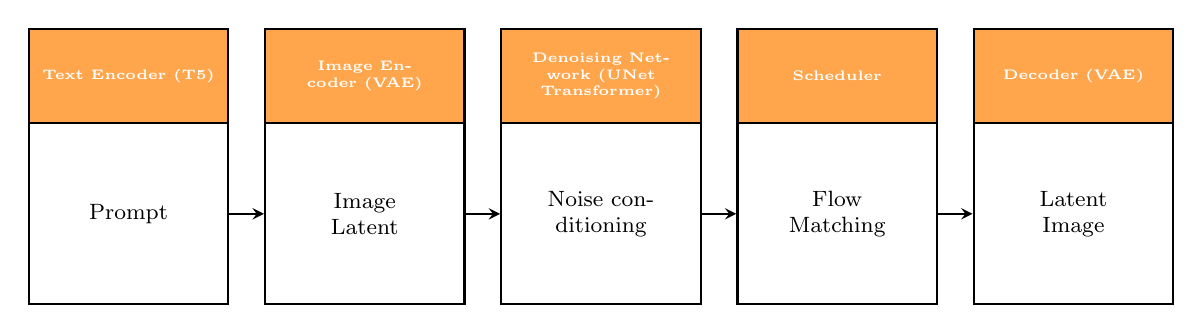
\begin{tikzpicture}[
    main_block/.style={
        rectangle,
        draw=black,
        thick,
        minimum width=2.5cm,
        minimum height=3.5cm,
        fill=white
    },
    header/.style={
        rectangle,
        draw=black,
        thick,
        minimum width=2.5cm,
        minimum height=1.2cm,
        fill=orange!70,
        text=white,
        font=\tiny\bfseries,
        align=center,
        text width=2.3cm
    },
    content/.style={
        rectangle,
        draw=black,
        thick,
        minimum width=2.5cm,
        minimum height=2.3cm,
        fill=white,
        font=\footnotesize,
        align=center,
        text width=2.3cm
    },
    arrow/.style={
        ->,
        thick,
        >=stealth
    }
]

\coordinate (pos1) at (0, 0);
\coordinate (pos2) at (3, 0);
\coordinate (pos3) at (6, 0);
\coordinate (pos4) at (9, 0);
\coordinate (pos5) at (12, 0);

\node[header] (h1) at (pos1) {Text Encoder (T5)};
\node[content] (c1) at ([yshift=-1.75cm]pos1) {Prompt};

\node[header] (h2) at (pos2) {Image Encoder (VAE)};
\node[content] (c2) at ([yshift=-1.75cm]pos2) {Image\\Latent};

\node[header] (h3) at (pos3) {Denoising Network (UNet Transformer)};
\node[content] (c3) at ([yshift=-1.75cm]pos3) {Noise conditioning};

\node[header] (h4) at (pos4) {Scheduler};
\node[content] (c4) at ([yshift=-1.75cm]pos4) {Flow\\Matching};

\node[header] (h5) at (pos5) {Decoder (VAE)};
\node[content] (c5) at ([yshift=-1.75cm]pos5) {Latent\\Image};

\draw[arrow] (c1.east) -- (c2.west);
\draw[arrow] (c2.east) -- (c3.west);
\draw[arrow] (c3.east) -- (c4.west);
\draw[arrow] (c4.east) -- (c5.west);

\end{tikzpicture}}
    \caption{Schema della pipeline del modello di Stable Diffusion 3.}
\end{figure}

